% Created 2023-09-08 Fri 10:03
% Intended LaTeX compiler: pdflatex
\documentclass[smaller]{beamer}\usepackage{listings}
\usepackage{color}
\usepackage{amsmath}
\usepackage{array}
\usepackage[T1]{fontenc}
\usepackage{natbib}
\lstset{
keywordstyle=\color{blue},
commentstyle=\color{red},stringstyle=\color[rgb]{0,.5,0},
literate={~}{$\sim$}{1},
basicstyle=\ttfamily\small,
columns=fullflexible,
breaklines=true,
breakatwhitespace=false,
numbers=left,
numberstyle=\ttfamily\tiny\color{gray},
stepnumber=1,
numbersep=10pt,
backgroundcolor=\color{white},
tabsize=4,
keepspaces=true,
showspaces=false,
showstringspaces=false,
xleftmargin=.23in,
frame=single,
basewidth={0.5em,0.4em},
}
\usepackage{natbib, dsfont, pgfpages, tikz,amssymb, amsmath,xcolor}
\bibliographystyle{abbrvnat}
% New operators and commands
\newcommand{\Z}{\mathbb{Z}}
\newcommand{\Q}{\mathbb{Q}}
\newcommand{\R}{\mathbb{R}}
\newcommand{\N}{\mathbb{N}}
\newcommand{\C}{\mathbb{C}}
\renewcommand{\S}{\mathbb{S}}
\newcommand{\blank}{\makebox[1ex]{\textbf{$\cdot$}}}
\newcommand\independent{\protect\mathpalette{\protect\independenT}{\perp}}
\def\independenT#1#2{\mathrel{\rlap{$#1#2$}\mkern2mu{#1#2}}}
\renewcommand{\phi}{\varphi}
\renewcommand{\epsilon}{\varepsilon}
\newcommand*\diff{\mathop{}\!\mathrm{d}}
\newcommand{\weakly}{\rightsquigarrow}
\newcommand\smallO{
  \mathchoice
    {{\scriptstyle\mathcal{O}}}% \displaystyle
    {{\scriptstyle\mathcal{O}}}% \textstyle
    {{\scriptscriptstyle\mathcal{O}}}% \scriptstyle
    {\scalebox{.6}{$\scriptscriptstyle\mathcal{O}$}}%\scriptscriptstyle
}
\newcommand{\midd}{\; \middle|\;}
\newcommand{\1}{\mathds{1}}
\usepackage{ifthen} %% Empirical process with default argument
% \newcommand{\G}[1][]{%
%    \ifthenelse{ \equal{#1}{} }
%       {\ensuremath{\mathbb{G}_n}}
%       {\ensuremath{\mathbb{G}_{#1}}}
% }
% New version:
\newcommand{\G}[2][n]{
{\ensuremath{\mathbb{G}_{#1}}{\left[#2\right]}}
}
\DeclareMathOperator*{\argmin}{\arg\!\min}

% New operators for consistent notation
\newcommand{\V}{\mathrm{Var}} % variance
\newcommand{\measure}[1]{\mathrm{{#1}}} % measure
% \newcommand{\measure}[1]{\textnormal{\textbf{{#1}}}} % measure
\newcommand{\m}[1]{\measure{#1}} % measure shortcut
\newcommand{\eqd}{\stackrel{d}{=}} % equality in distribution
\newcommand{\arrow}[1]{\xrightarrow{\; {#1} \;}}
\newcommand{\arrowP}{\xrightarrow{\; \m{P} \;}} % convergence in probability
\newcommand{\leb}{\lambda} % the Lebesgue measure
\newcommand{\T}{\top} % transpose
\newcommand{\KL}{\ensuremath{D_{\mathrm{KL}}}}

\usepackage{xargs}
% Make it easy to change counterfactual notation:
\newcommandx{\cf}[4][3={}, 4={}]{
  % \ifthenelse{ \equal{#4}{} }
  % {{#1^{#2}}(#3)}
  {\ifthenelse{ \equal{#3}{} }
    {{#1^{#2}}_{#4}}
    {{#1^{#2}}_{#4}(#3)}}
}

% Easily change notation:
\DeclareMathOperator{\TT}{\Psi} % target parameter
\newcommand{\lp}{\mathcal{L}_{\P}^2} % shortcut for lp2 space
\newcommand{\empmeas}{\hat{\mathbb{P}}_n} % empirical measure
\DeclareMathOperator{\E}{\mathbb{E}} % expectation
\renewcommand{\P}{\m{P}} % probability
\newcommand{\ic}{\mathrm{IF}} % influence curve
\setbeamertemplate{footline}[frame number]
\beamertemplatenavigationsymbolsempty
\usepackage{appendixnumberbeamer}
\setbeamercolor{gray}{bg=white!90!black}
\setbeamertemplate{itemize items}{$\circ$}

\renewcommand*\familydefault{\sfdefault}
\itemsep2pt
\usepackage[utf8]{inputenc}
\usepackage[T1]{fontenc}
\usepackage{graphicx}
\usepackage{longtable}
\usepackage{wrapfig}
\usepackage{rotating}
\usepackage[normalem]{ulem}
\usepackage{amsmath}
\usepackage{amssymb}
\usepackage{capt-of}
\usepackage{hyperref}
\usetheme{default}
\author{Anders Munch and Thomas Gerds}
\date{September 11, 2023}
\title{Targeted learning under shape constraints}
\begin{document}

\maketitle
\begin{frame}[label={sec:org20ef451}]{Motivation}
The road map of causal learning tells us to incorporate all the knowledge that we have
  into the statistical model for the distribution of the data
\vfill

In many real applications, subject matter knowledge is available
  regarding the shape of the underlying conditional density and
  regression functions
\vfill

Examples of biologically motivated shapes are
\begin{itemize}
\item risk of disease is not decreasing with age (given other covariates)
\item The risk of disease should be a monotone function of age (given other covariates)
\item The number of comorbidities increases the risk of disease
\item the effect of a biomarker on the risk of disease is an unimodal function (given other covariates)
\end{itemize}
\end{frame}

\begin{frame}[label={sec:org7a57632}]{Target and nuisance parameters}
Consider a real-valued target parameter \(\psi: \mathcal P\to\R\) 

\begin{equation*}
\psi(\mathrm P_{Q,G}) = \nu(Q)
\end{equation*}

for some functional \(\nu:\mathcal Q\to\R\) such that \(G\) and 'all
other parts' of \(Q\) are nuisance parameters.
\vfill

Shape constraints on a function-valued target parameter have been
considered by many, e.g.,
\citet[][]{groeneboom2014nonparametric,westling2020unified,wu2022nonparametric}. 
\vfill

Today, we will mostly discuss imposing shape-constraints on nuisance
parameters.
\end{frame}

\begin{frame}[label={sec:orgbc0ca9d}]{}
\begin{block}{Working hypotheses}
\begin{itemize}
\item Shape constraints can be incorporated into machine learning for nuisance parameters
\item Biologically motivated shape constraints 
may lead to improved estimators
\end{itemize}

\vspace{4em}
\end{block}

\begin{block}{Goal for the workshop}
\begin{itemize}
\item Discuss some initial hypotheses and ideas
\item Help us move in the right research direction
\end{itemize}
\end{block}
\end{frame}

\begin{frame}[label={sec:org2df52a4}]{Multivariate shape constraints}
\begin{figure}[htbp]
\centering
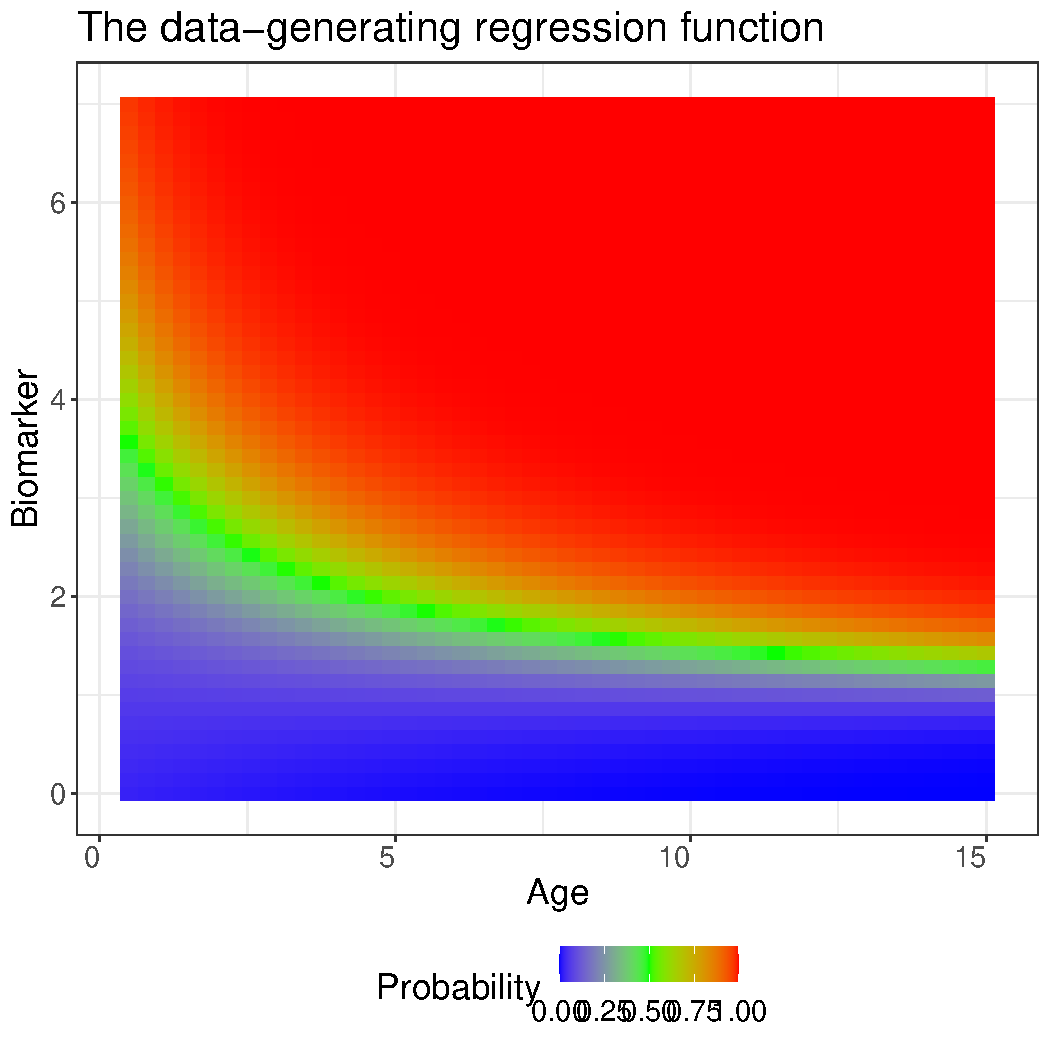
\includegraphics[width=0.7\textwidth]{./a.pdf}
\label{fig:1}
\end{figure}
\end{frame}

\begin{frame}[label={sec:org21dcf35}]{Machine learning (from the shelf)}
\begin{figure}[htbp]
\centering
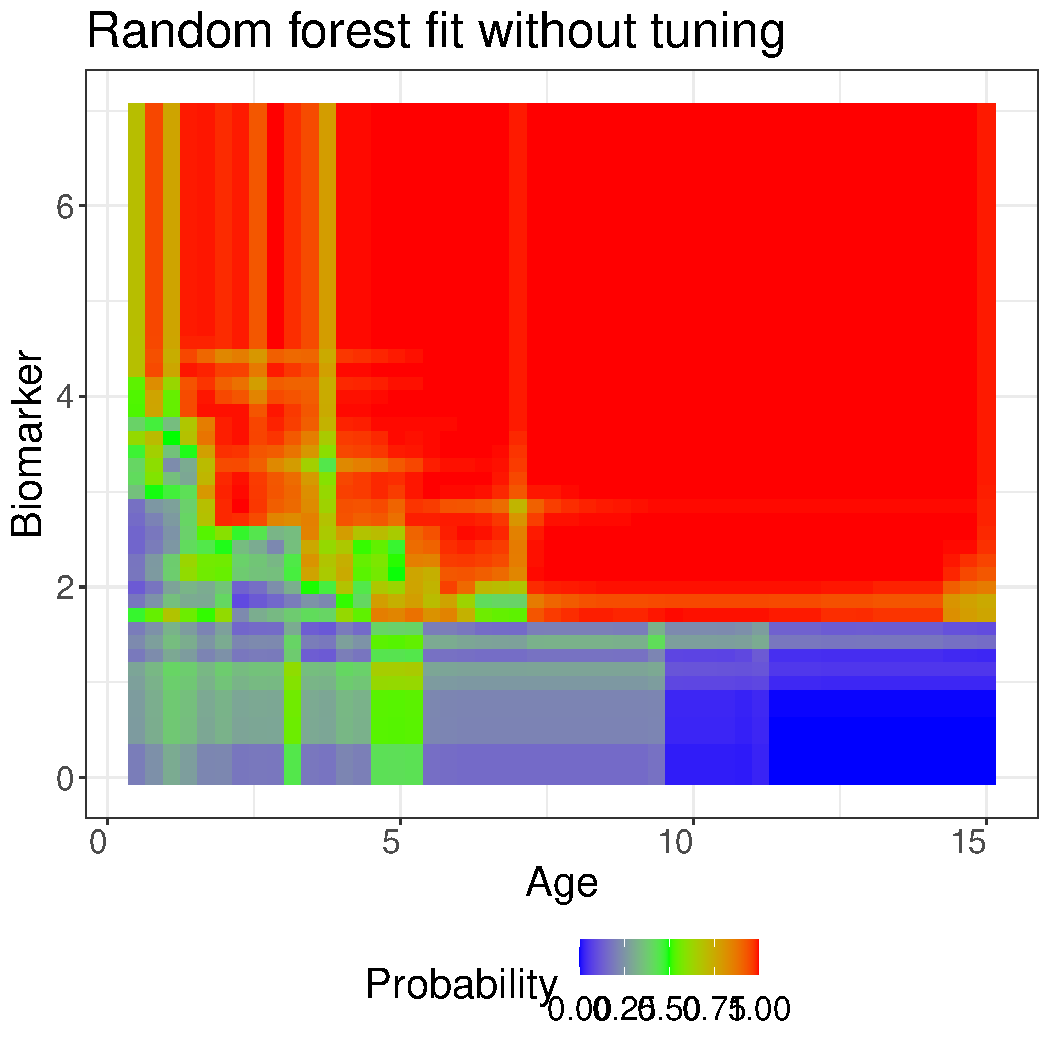
\includegraphics[width=0.7\textwidth]{./b.pdf}
\label{fig:1}
\end{figure}
\end{frame}
\begin{frame}[label={sec:org8ef1209}]{Shape constraints}
\begin{block}{Examples}
\begin{itemize}
\item Monotonicity
\item Unimodality
\item Convexity
\item Log-concave density
\end{itemize}
\end{block}

\begin{block}{Tools to incorporate shape constraints into machine learning}
\begin{itemize}
\item Model specification/architecture
\item Internal parameter tuning
\item External penalty/loss function
\item Smoothing applied to the fitted object
\item Log-concave sampling
\item what else?
\end{itemize}
\end{block}
\end{frame}

\begin{frame}[label={sec:orgb9ccb59}]{Information bounds}
\begin{alertblock}{Conjecture 1}
Some shape constraints will not restrict the tangent space, and hence
imposing such shape constraints does not change the information bound
for the statistical estimation problem.

\begin{itemize}
\item Which shape constraints satisfy this when imposed on G and/or Q?
\item Can we still improve a targeted minimum loss estimator (TMLE) by
imposing such shape constraints on the nuisance parameters?
\end{itemize}
\end{alertblock}

\begin{alertblock}{Conjecture 2}
Constructing a TMLE under a shape constrained model will typically result in a
sub-model that is not contained in the shape constrained model (c.f.,
\cite{van1989asymptotic}).
\end{alertblock}

\begin{alertblock}{Conjecture 3}
Imposing shape constraints can improve the convergence rates of
machine learning.
\end{alertblock}
\end{frame}

\begin{frame}[label={sec:orgb1b9ec5}]{(Un)necessary restrictions on nuisance parameters?}
\begin{block}{Undersmoothing}
It has been shown that undersmoothing of the estimators of the
nuisance parameters is needed when they are 'plugged-in' to estimate a
low-dimensional target parameter
\citep[e.g.,][]{goldstein1996efficient,hjort2001note,van2022efficient}.
\vspace{1em}

\alert{Could shape constraints induce unnecessary/unfortunate smoothing?}
\end{block}


\begin{block}{Biologically reasonable nuisance parameter estimators?}
Should we pay attention to whether nuisance parameters are estimated
by biologically meaningful estimators? \vspace{1em}

Should we accept a biologically unreasonable estimator of a nuisance parameter
as long as it provides a good estimator of the target parameter?
\end{block}
\end{frame}


\begin{frame}[label={sec:org0b2146b}]{Estimating a cumulative distribution function}
\small

\begin{description}
\item[{\color{red}ECDF}] Empirical distribution function
\item[{\color{orange}kernCDF}] Estimator based on smoothed kernel density estimator
\item[{\color{blue}logConCDF}] Estimator based on log-concave density estimator
\citep{dumbgen2009maximum,Rufibach_Duembgen_2023}
\end{description}

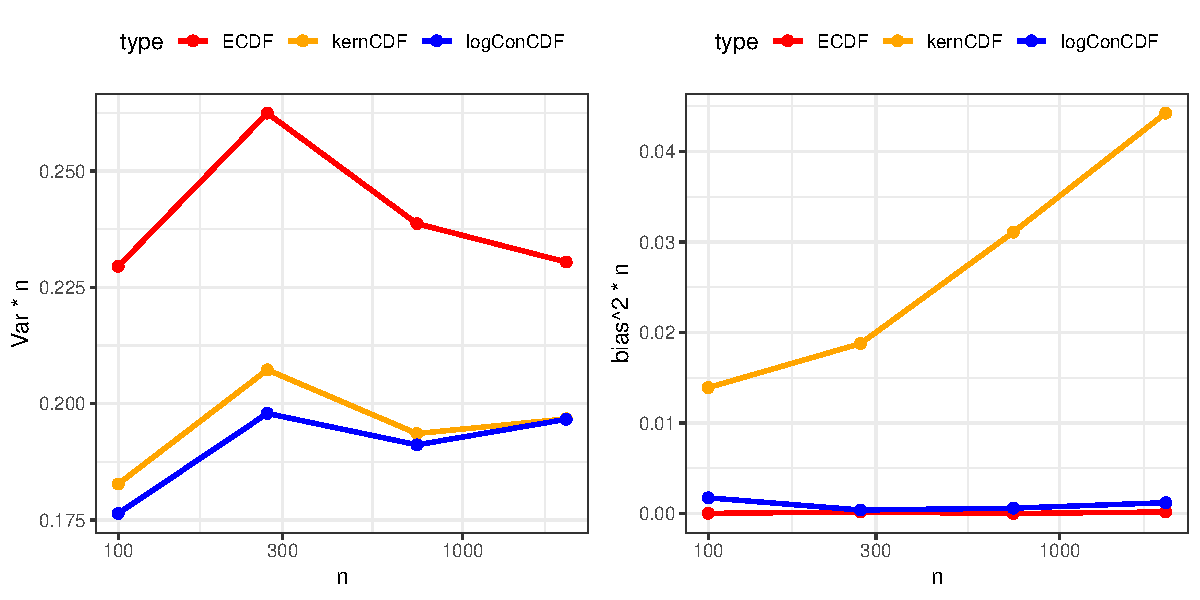
\includegraphics[width=1\textwidth]{./cdf-estimators.pdf}
\end{frame}


\begin{frame}[label={sec:orga8e14be}]{Challenges for future research}
\begin{itemize}
\item Should we distinguish between learning Q vs G parts of a causal
model/information loss model?

\item How do we translate ``marginal'' smoothness constraints into 
constraints on a multivariate function?

\item In longitudinal settings, need to discuss shape-constraints on the
history (filtration): an older value of a variable (such as A1c in
diabetes) should have a lower effect than a newer value of the same
variable.
\end{itemize}
\end{frame}

\begin{frame}[label={sec:org619d706}]{References}
\footnotesize \bibliography{./latex-settings/default-bib.bib}
\end{frame}
\end{document}